%\clearpage

\appendix
\renewcommand{\appendixname}{Anexos}
\renewcommand{\appendixtocname}{Anexos}
\renewcommand{\appendixpagename}{Anexos}
\clearpage
\addappheadtotoc
%\appendixpage %Agrega una pagina en blanco q en el medio Dice Anexo en grande..



    \begin{minipage}{0.95\textwidth}
    \chapter{Diagrama del modelo de casos de uso}
    %\section{Diagrama del modelo de casos de uso}
    	\leftline{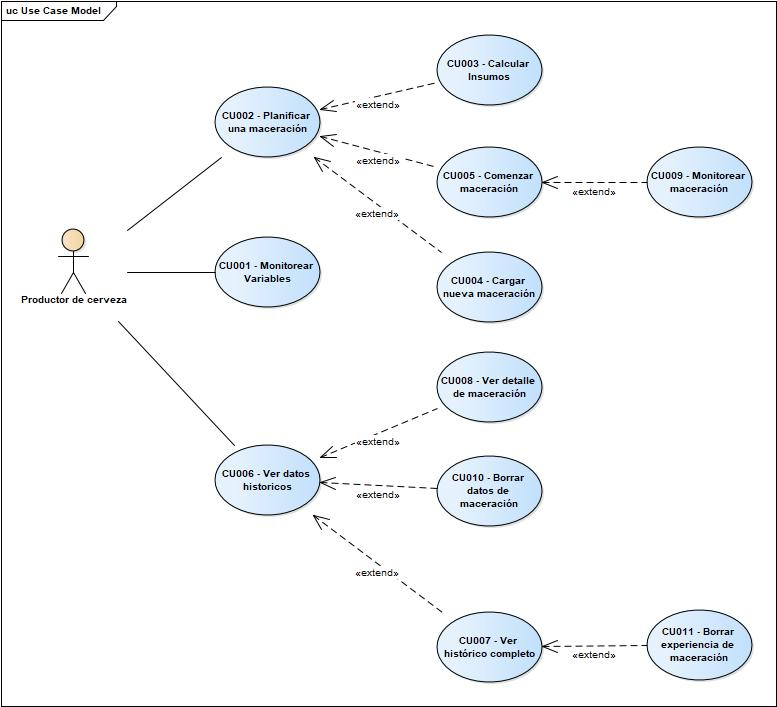
\includegraphics[scale=0.55]{ModelodeCasosdeUso.jpg}}
    	\captionof{figure}{Diagrama de Casos de Uso}
	    \label{DiagCU}
	\end{minipage}


    \begin{minipage}{0.95\textwidth}
    \chapter{Diagrama de base de datos del componente de Hardware}
        \centering
        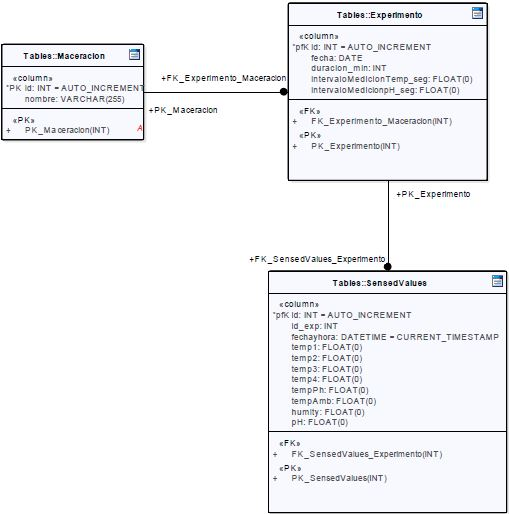
\includegraphics[scale=1]{diagramaBD-Rasp.jpg}
        \captionof{figure}{Diagrama de diseño de Base de Datos}
        \label{fig:DiagramaBdRasp}
    
    \end{minipage}
    
    \begin{minipage}{0.95\textwidth}
    \chapter{Esquema de conexión de la estación de recolección de datos}
        \centering
        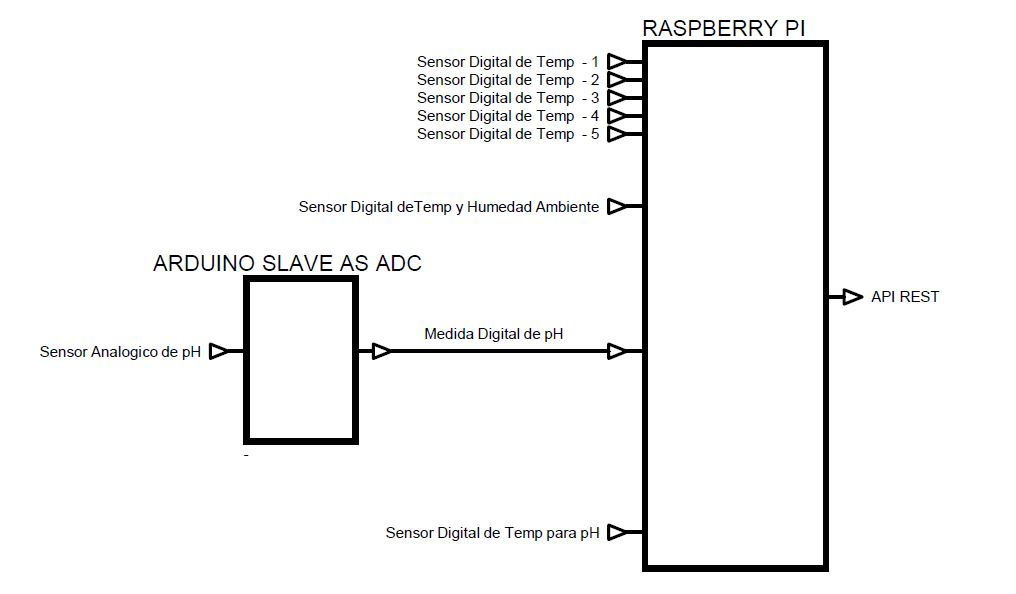
\includegraphics[scale=0.55]{EsquemaHardware.jpg}
        \captionof{figure}{Esquema simplificado de las conexiones}
        \label{fig:EsquemaHardware}
    \end{minipage}
    
%---------------------- MOCK UP ----------------------------------------
    \begin{minipage}{0.95\textwidth}
    \chapter{Diseño de Interfaz de Usuario}
    %\section{Diseño de Interfaz de Usuario}
        \centering
        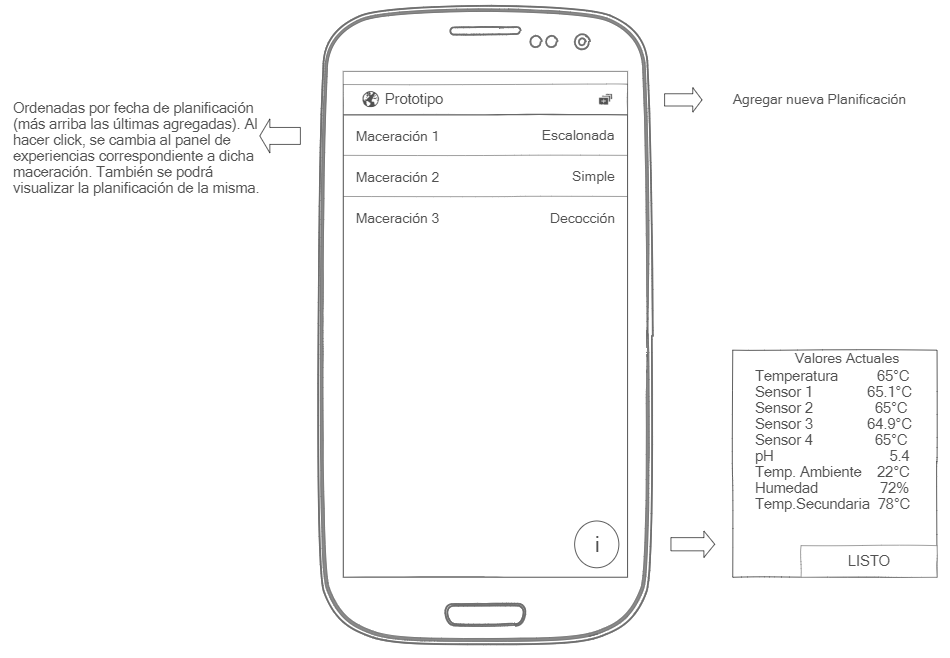
\includegraphics[scale=0.55]{Anexo/MockUp/MainActivity.jpg}
        \captionof{figure}{Pantalla Principal}
        \label{fig:MockUpMainActivity}
    \end{minipage}
    
    \begin{minipage}{0.95\textwidth}

        \centering
        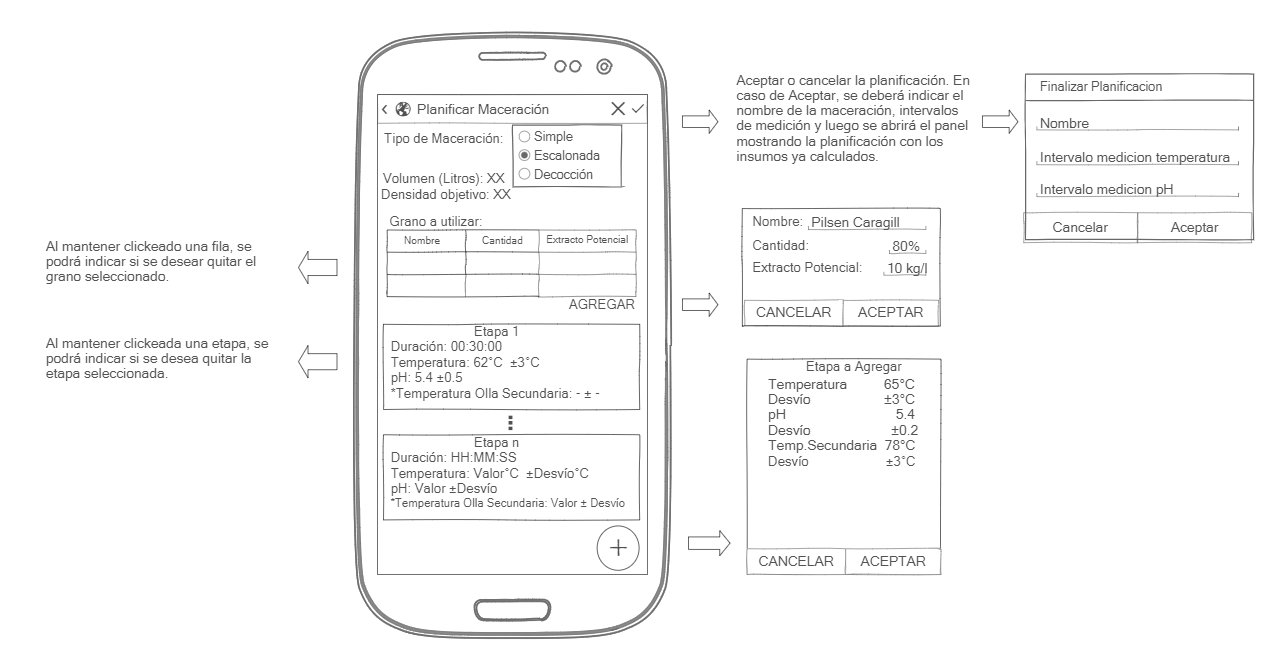
\includegraphics[scale=0.55, angle =90]{Anexo/MockUp/PlanningActivity.jpg}
        \captionof{figure}{Pantalla de planificación de maceración}
        \label{fig:MockUpPlanningActivity}
    \end{minipage}
    
    \begin{minipage}{0.95\textwidth}

        \centering
        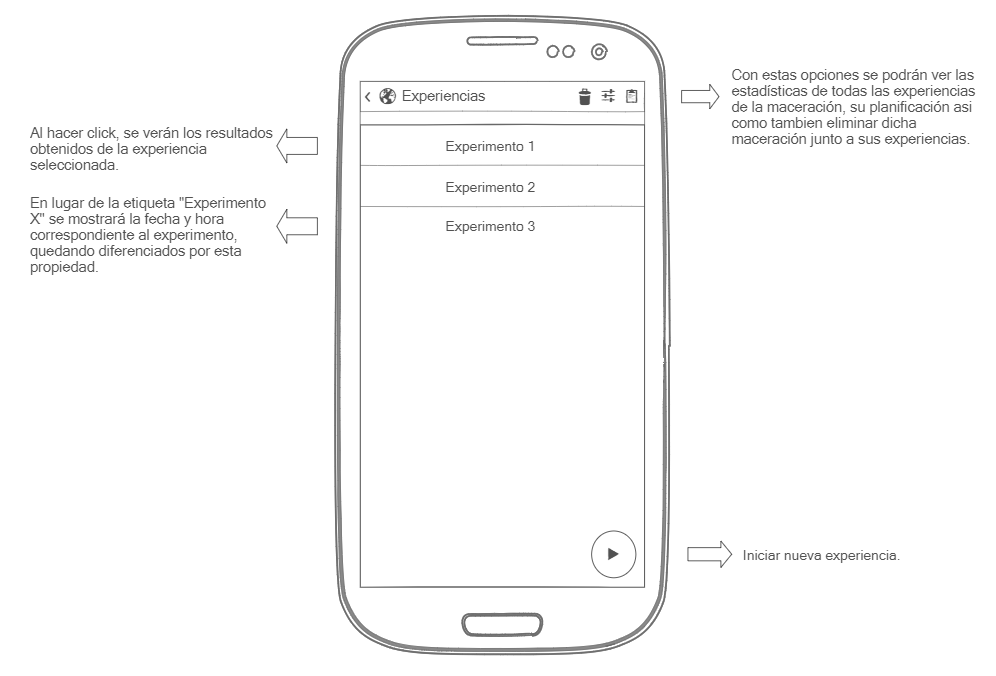
\includegraphics[scale=0.55]{Anexo/MockUp/ExperimentActivity.jpg}
        \captionof{figure}{Pantalla con lista de experimentos de una maceración}
        \label{fig:MockUpExperimentActivity}
    \end{minipage}
    
    \begin{minipage}{0.95\textwidth}

        \centering
        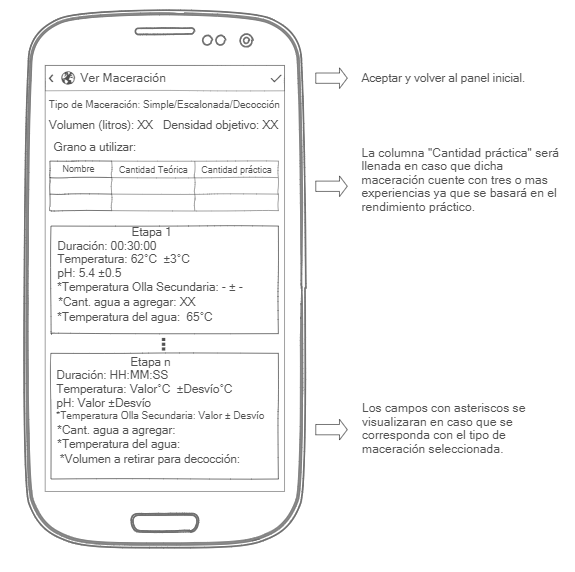
\includegraphics[scale=0.7]{Anexo/MockUp/InfoMash.jpg}
        \captionof{figure}{Pantalla con información de la maceración}
        \label{fig:MockUpInfoMash}
    \end{minipage}
    
    \begin{minipage}{0.95\textwidth}

        \centering
        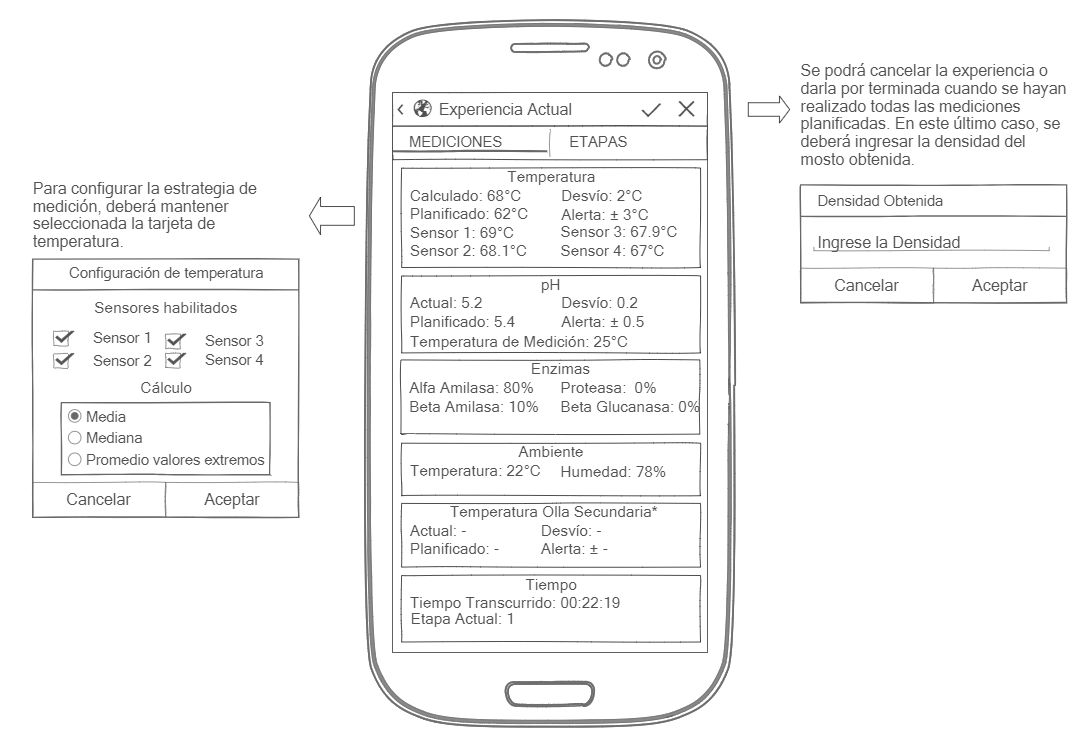
\includegraphics[scale=0.5]{Anexo/MockUp/CurrentExperience-MeasureFragment.jpg}
        \captionof{figure}{Pantalla de mediciones del experimento en ejecución}
        \label{fig:MockUpCurrentExperienceFragment}
    \end{minipage}
    
    \begin{minipage}{0.95\textwidth}

        \centering
        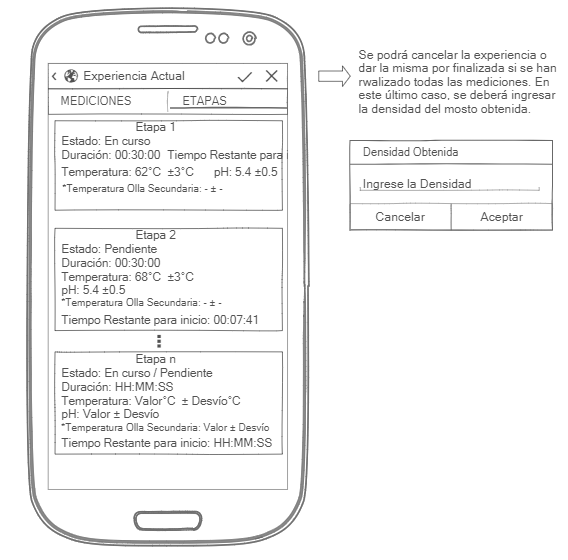
\includegraphics[scale=0.7]{Anexo/MockUp/CurrentExperience-StageFragment.jpg}
        \captionof{figure}{Pantalla con información de las etapas del experimento en ejecución}
        \label{fig:MockUpStageFragment}
    \end{minipage}
    
    \begin{minipage}{0.95\textwidth}

        \centering
        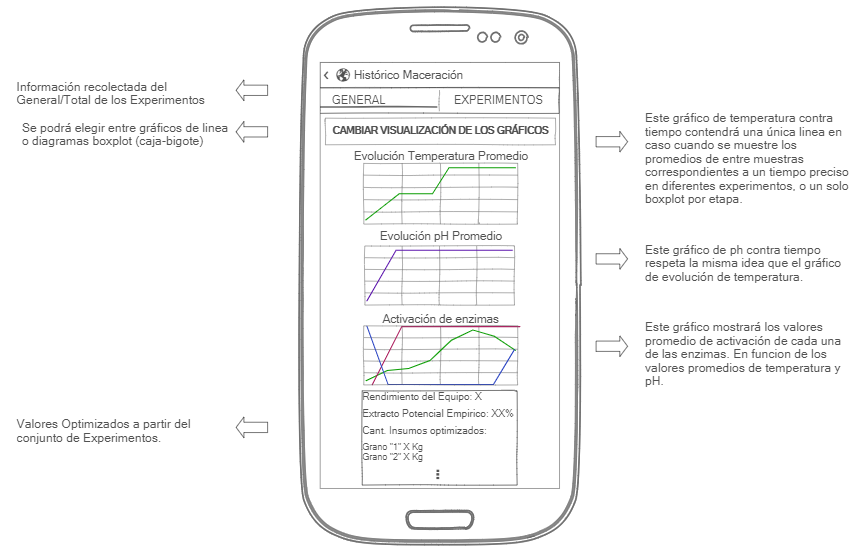
\includegraphics[scale=0.7]{Anexo/MockUp/MashExpHistoryActivity-GeneralFragment.jpg}
        \captionof{figure}{Pantalla con información estadística descriptiva de mediciones y de optimización de insumos y rendimiento}
        \label{fig:MockUpGeneralFragment}
    \end{minipage}
    
    \begin{minipage}{0.95\textwidth}

        \centering
        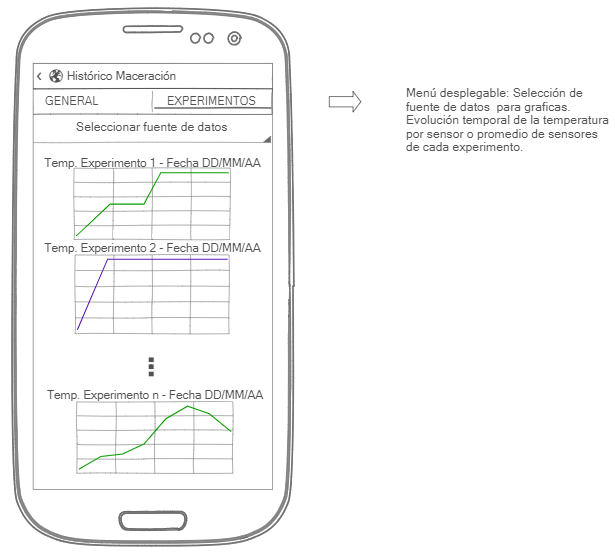
\includegraphics[scale=0.7]{Anexo/MockUp/MashExpHistoryActivity-ExperimentFragment.jpg}
        \captionof{figure}{Pantalla con información estadística descriptiva de mediciones de temperatura de cada experimento}
        \label{fig:MockUpExperimentFragment}
    \end{minipage}
    
   \begin{minipage}{0.95\textwidth}

        \centering
        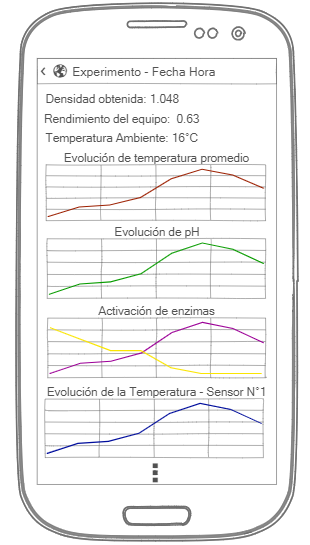
\includegraphics[scale=0.7]{Anexo/MockUp/DetailExperimentActivity.jpg}
        \captionof{figure}{Pantalla con información detalladas de los resultados de cada experimento}
        \label{fig:MockUpDetailExperimentActivity}
    \end{minipage}
    
%-------------------------- DIAGRAMAS DE CLASE --------------------------- 
    \begin{minipage}{0.95\textwidth}
    \chapter{Diagramas de clases}
    %\begin{figure}
        \centering
        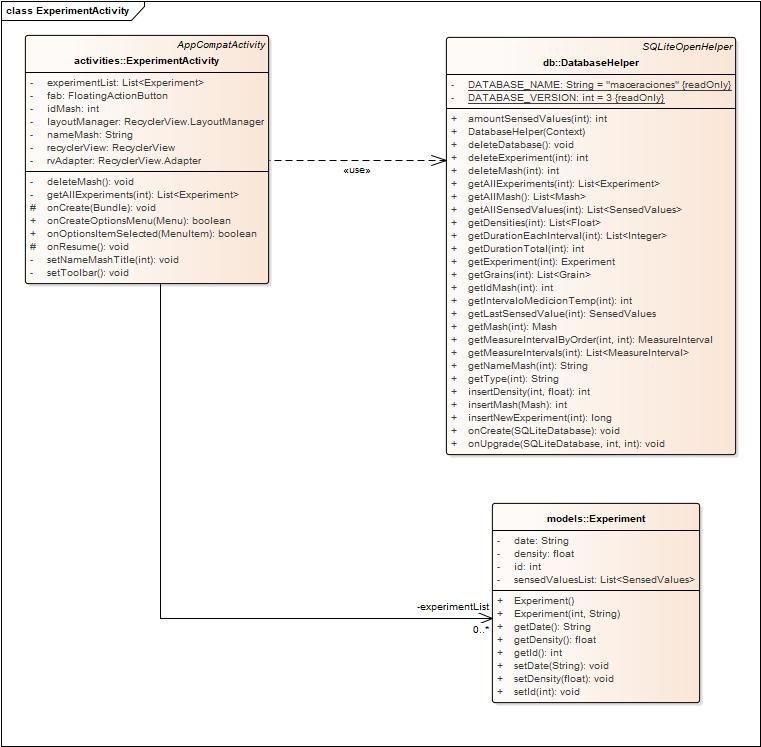
\includegraphics[scale=0.55, angle=90]{Anexo/DiagramasClase/ExperimentActivity.jpg}
        \captionof{figure}{Diagrama de clases de ExperimentActivity}
        \label{fig:DiagClaseExperimentActivity}
    %\end{figure}
    \end{minipage}
    
    %\begin{minipage}{0.95\textwidth}
            \begin{figure}
                \centering
                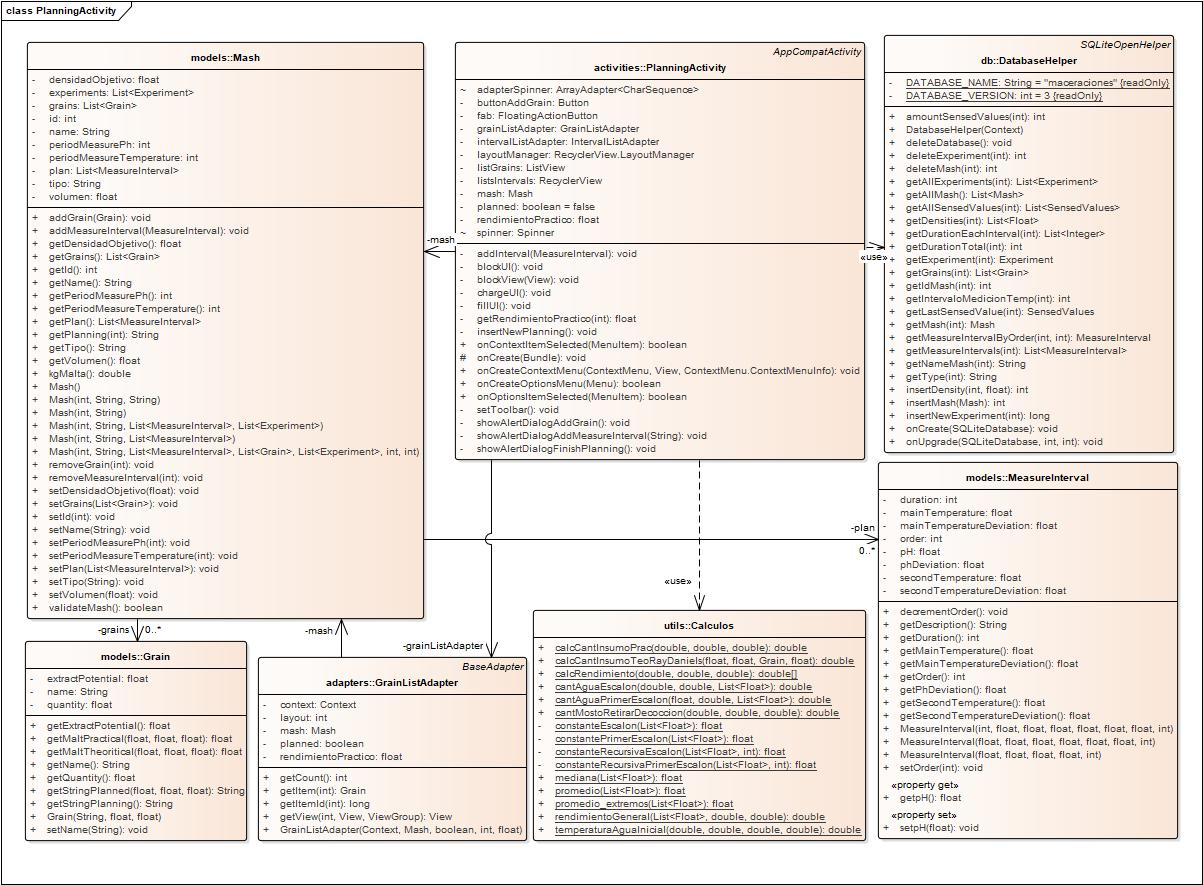
\includegraphics[scale=0.5, angle=90]{Anexo/DiagramasClase/PlanningActivity.jpg}
                \captionof{figure}{Diagrama de clases de PlanningActivity}
                \label{fig:DiagClasePlanningActivity}
            \end{figure}
    %\end{minipage}
    
    
    \begin{figure}
        %\section{Diagramas de clases}
        \centering
        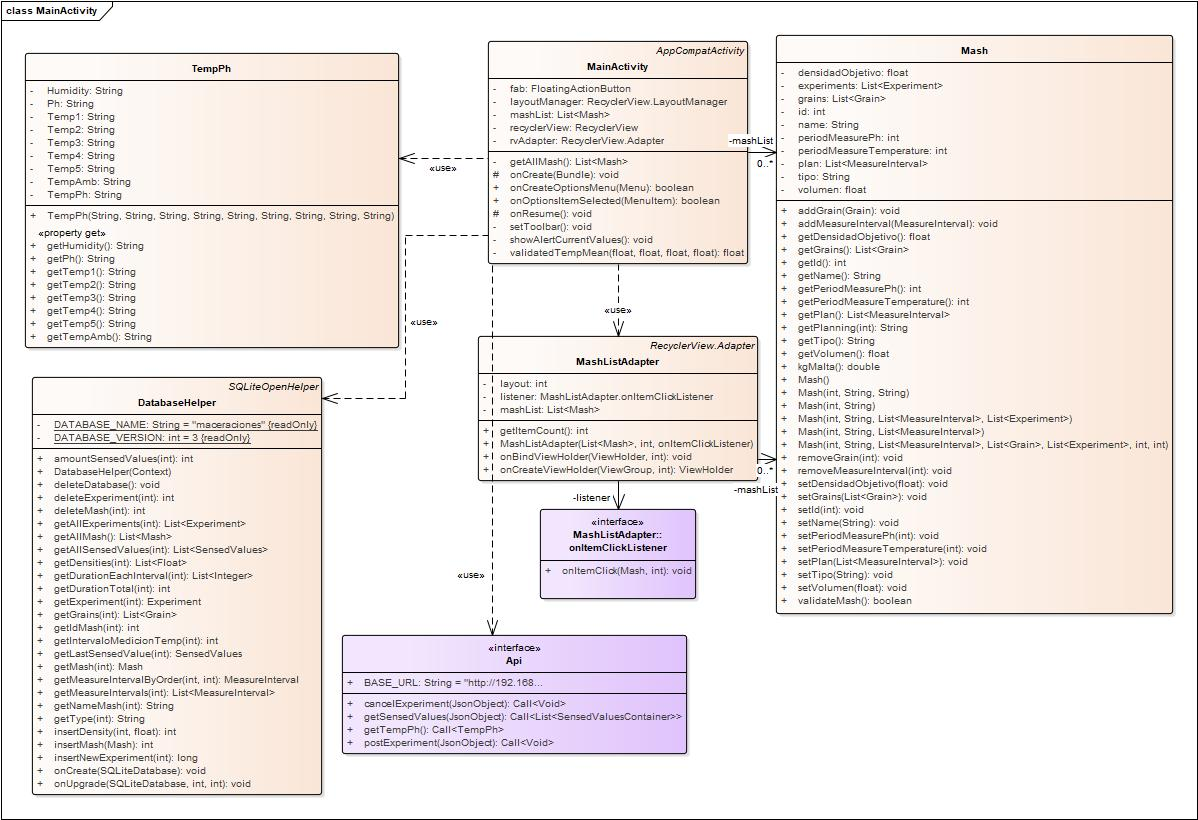
\includegraphics[scale=0.5, angle =90]{Anexo/DiagramasClase/MainActivity.jpg}
        \captionof{figure}{Diagrama de clases de MainActivity}
        \label{fig:DiagClaseMainActivity}
    \end{figure}
    
    
    %\begin{minipage}{0.95\textwidth}
    \begin{figure}
        \centering
        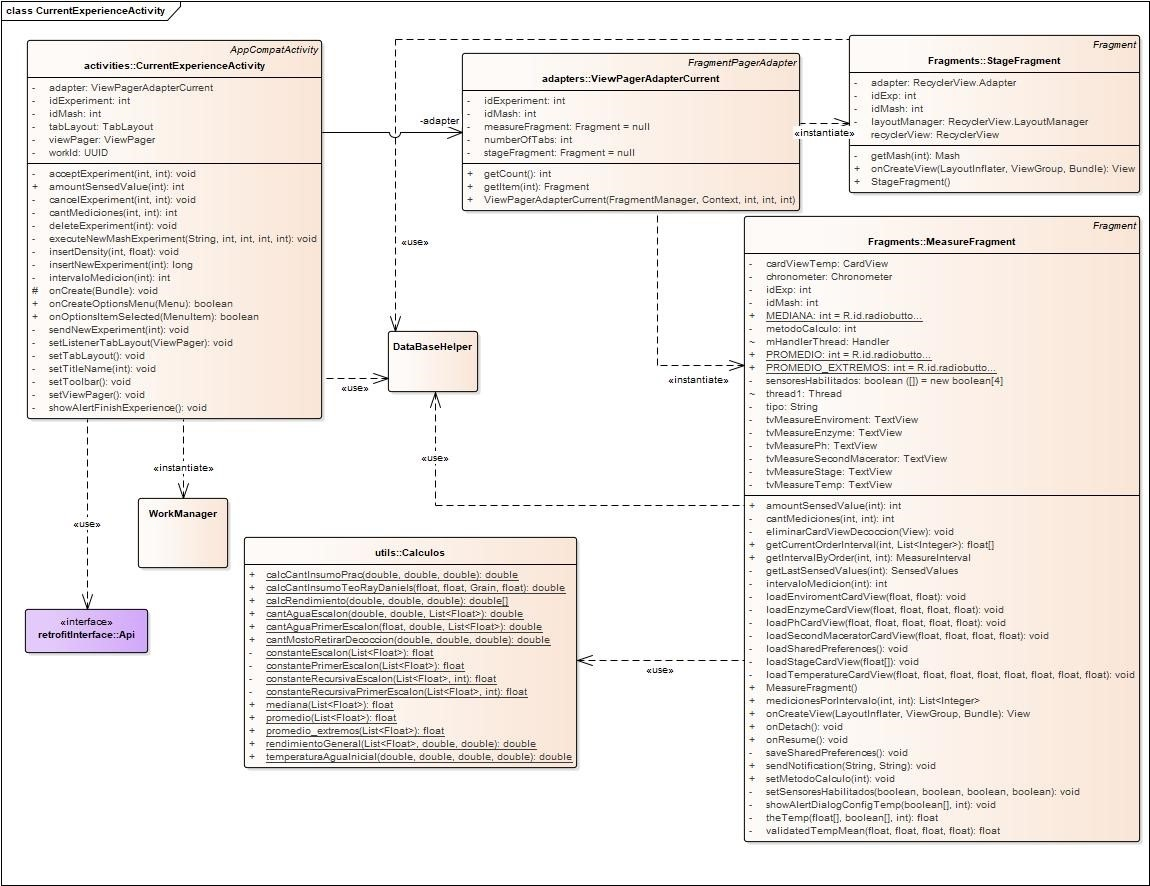
\includegraphics[scale=0.6, angle=90]{Anexo/DiagramasClase/CurrentExperienceActivity-P1.jpg}
        \captionof{figure}{Diagrama de clases de CurrentExperienceActivity - Parte 1}
        \label{fig:DiagClaseCurrentExperienceActivityP1}
    \end{figure}
    %\end{minipage}
    
    %\begin{minipage}{0.95\textwidth}
    \begin{figure}
        \centering
        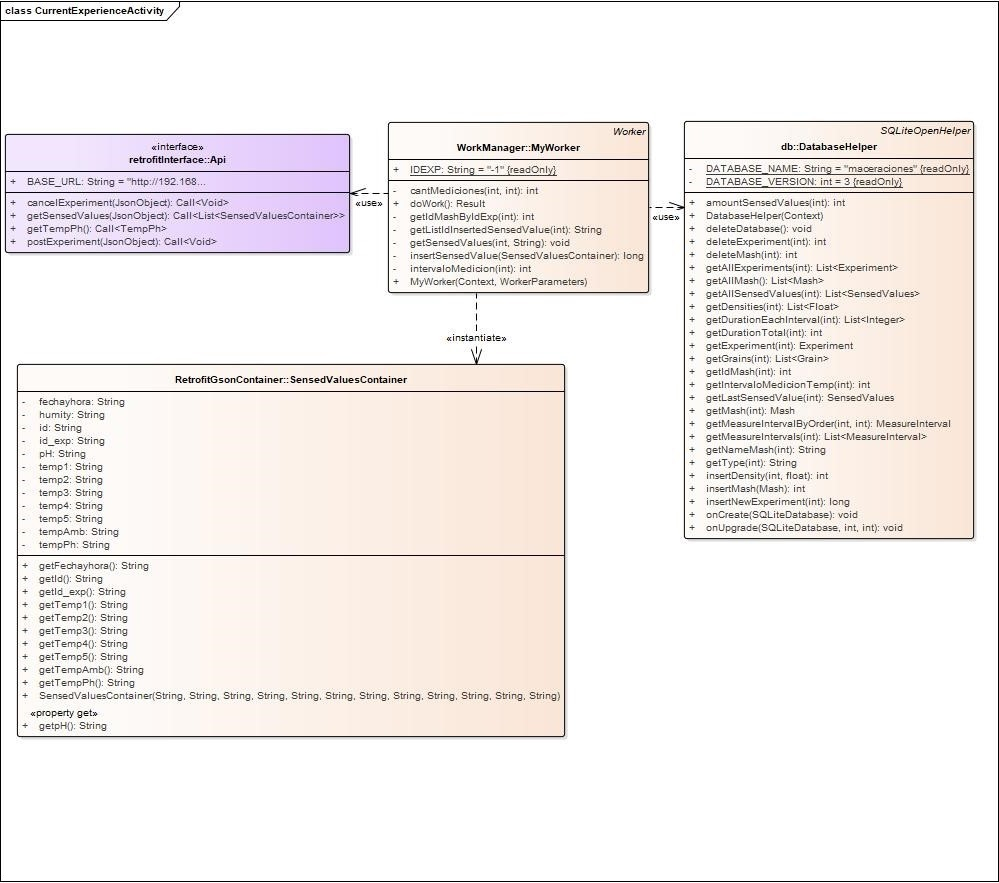
\includegraphics[scale=0.6, angle=90]{Anexo/DiagramasClase/CurrentExperienceActivity-P2.jpg}
        \captionof{figure}{Diagrama de clases de CurrentExperienceActivity - Parte 2}
        \label{fig:DiagClaseCurrentExperienceActivityP2}
    \end{figure}
    %\end{minipage}
    
    %\begin{minipage}{0.95\textwidth}
        \begin{figure}
        \centering
        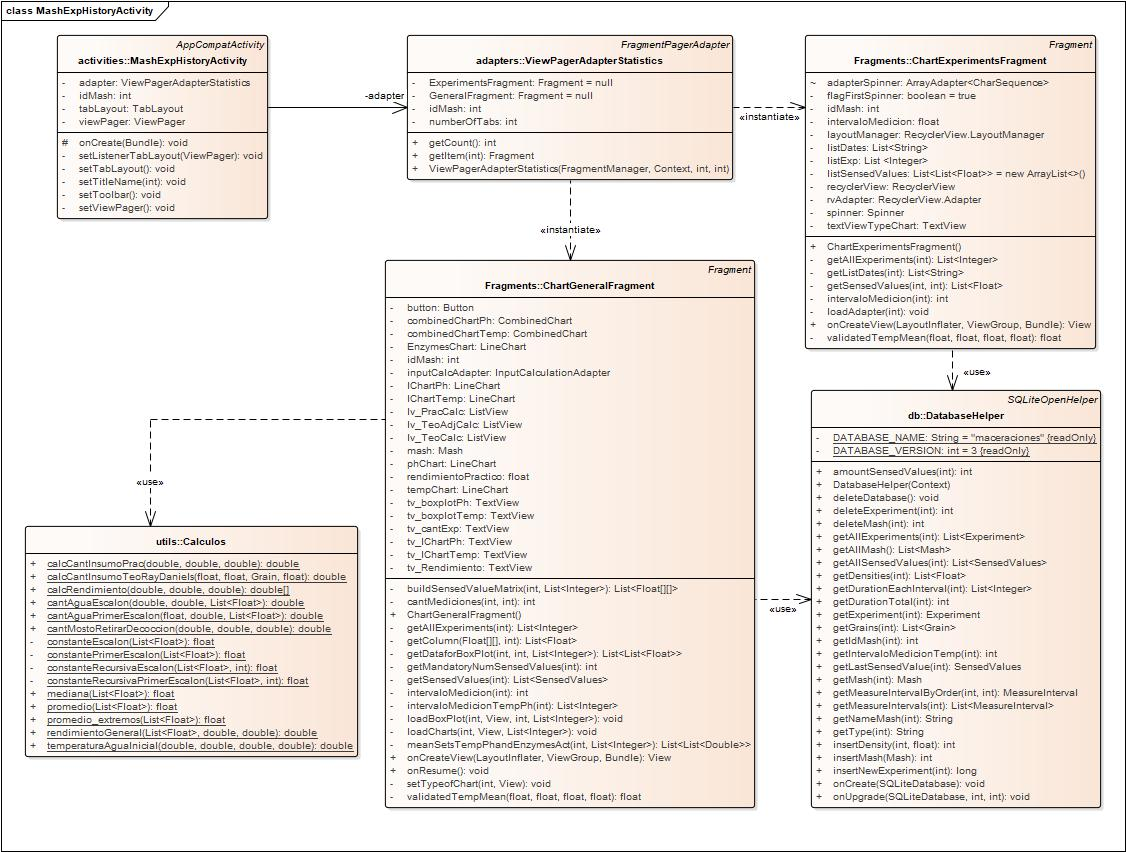
\includegraphics[scale=0.5, angle=90]{Anexo/DiagramasClase/MashExpHistoryActivity.jpg}
        \captionof{figure}{Diagrama de clases de MashExpHistoryActivity}
        \label{fig:DiagClaseMashExpHistoryActivity}
        \end{figure}
    %\end{minipage}
    
    %\begin{minipage}{0.95\textwidth}
        \begin{figure}
        \centering
        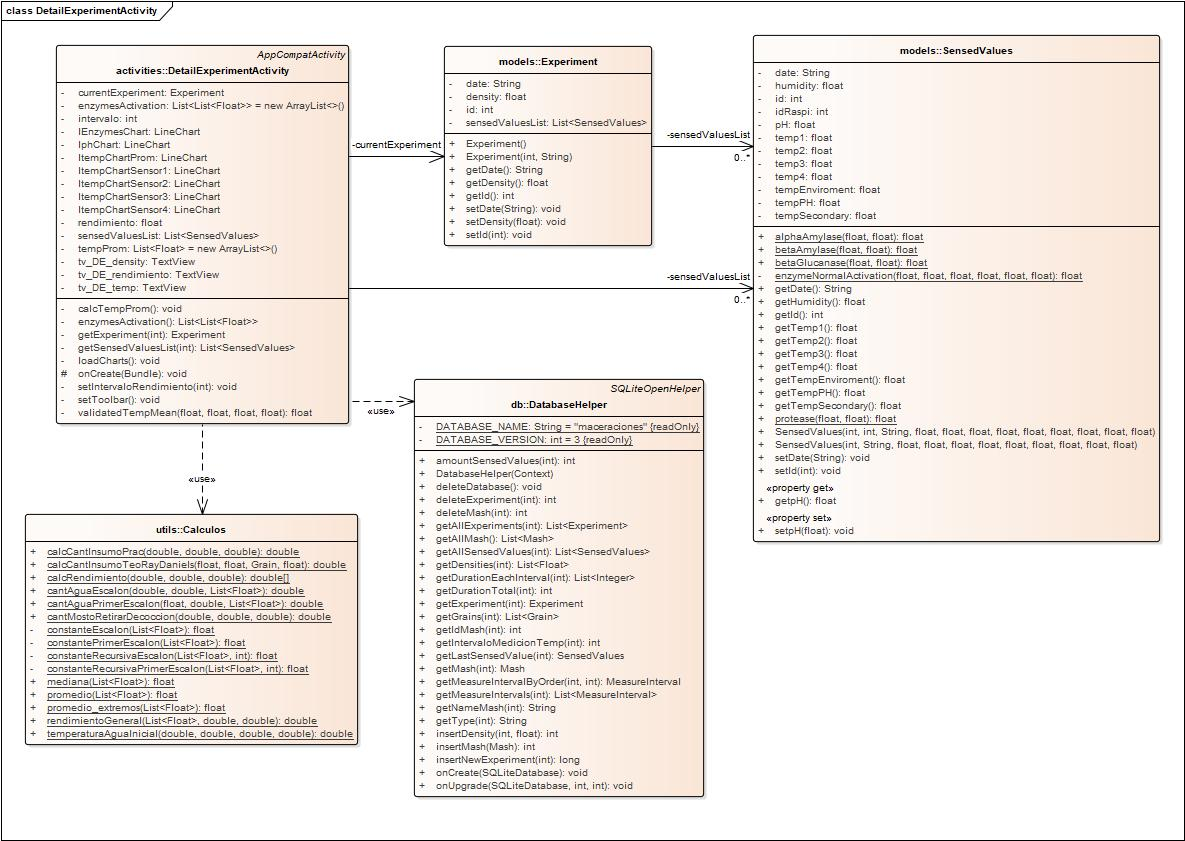
\includegraphics[scale=0.5, angle=90]{Anexo/DiagramasClase/DetailExperimentActivity.jpg}
        \captionof{figure}{Diagrama de clases de DetailExperimentActivity}
        \label{fig:DiagClaseDetailExperimentActivity}
        \end{figure}
    %\end{minipage}
    
    %\begin{minipage}{0.95\textwidth}
        \begin{figure}
        \centering
        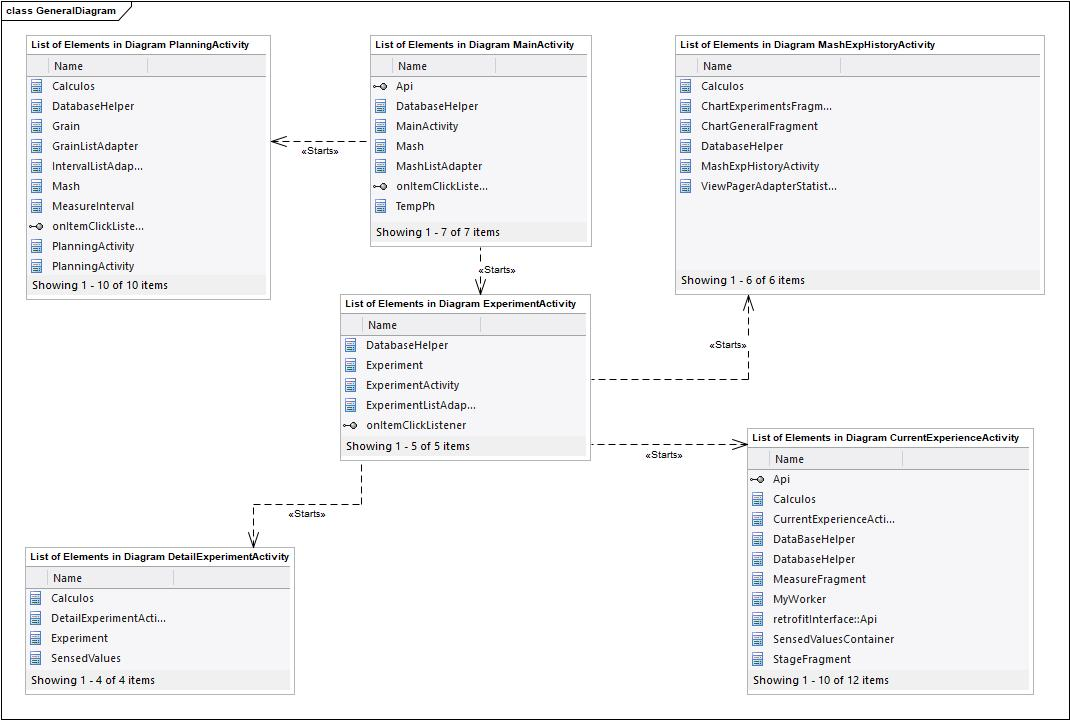
\includegraphics[scale=0.5, angle=90]{Anexo/DiagramasClase/GeneralDiagram.jpg}
        \captionof{figure}{Diagrama General de la APP}
        \label{fig:DiagGeneral}
        \end{figure}
    %\end{minipage}
    
    
    
    \begin{minipage}{0.95\textwidth}
    \subsection{Casos de Prueba}
    \label{CasosPrueba}
    \begin{center}
    \begin{tabularx}{\textwidth}{ | p{2cm} | X | X | X |}
        \hline
        \multicolumn{4}{|c|}{\textbf{Caso de Prueba: Monitorear variables - CP001}} \\
        \hline
        \multicolumn{4}{|l|}{\textbf{Actor Caso de Prueba:} Productor de Cerveza} \\
        \hline
        \multicolumn{4}{|l|}{\textbf{Propósito}} \\
        \hline
        \multicolumn{4}{|p{0.95\linewidth}|}{Verificar la correcta funcionalidad del dialogo que proporciona los datos siendo recolectados por los sensores de la estación de recolección de datos. Verificar que se despliegan en pantalla los datos antes mencionados} \\
        \hline
        \multicolumn{4}{|l|}{\textbf{Descripción de las acciones para las pruebas}} \\
        \hline
        \textbf{\#} & Acciones & Salida Esperada & Salida Obtenida \\
        \hline
        01 & Abrir el panel mediante el botón destinado a ello presente en la pantalla principal & Se abre el panel y se despliegan los datos esperados. & El panel se abrió correctamente y se mostraron luego los datos esperados. \\
        \hline
        \multicolumn{4}{|c|}{\textbf{Resultados Obtenidos}} \\
        \hline
        \multicolumn{4}{|l|}{\textbf{Resultado:} Aprobado} \\
        \hline
        \multicolumn{4}{|l|}{\textbf{Evidencia: }} \\
        \hline
     \end{tabularx}
    \label{CP001}
    \end{center}
    \end{minipage}
    
    \begin{minipage}{0.95\textwidth}
    \begin{center}
    \begin{tabularx}{\textwidth}{ | p{2cm} | X | X | X |}
        \hline
        \multicolumn{4}{|c|}{\textbf{Caso de Prueba: Planificar una maceración - CP002}} \\
        \hline
        \multicolumn{4}{|l|}{\textbf{Actor Caso de Prueba:} Productor de Cerveza} \\
        \hline
        \multicolumn{4}{|l|}{\textbf{Propósito}} \\
        \hline
        \multicolumn{4}{|p{0.95\linewidth}|}{Verificar la correcta apertura y funcionalidad de la pantalla destinada para la carga y creación de una nueva maceración.} \\
        \hline
        \multicolumn{4}{|l|}{\textbf{Descripción de las acciones para las pruebas}} \\
        \hline
        \textbf{\#} & Acciones & Salida Esperada & Salida Obtenida \\
        \hline
        01 & Apertura de la pantalla mediante el botón destinado a ello presente en la pantalla principal & Se abre la pantalla con el formulario. & La pantalla se abrió correctamente desplegando en ella el formulario a rellenar. \\
        \hline
        02 & Agregar grano (formulario incompleto), apertura del diálogo y relleno incompleto del formulario & Se abre el diálogo con el formulario. No se agrega el grano y despliega un mensaje de error. & Se abrió el diálogo con el formulario. No se agregó el grano y desplegó un mensaje de error:"No se pudo insertar el grano porque faltaron completar campos". \\
        \hline
        03 & Agregar grano (formulario completo), apertura del diálogo y relleno completo del formulario, luego se agrega el mismo pudiendo ver los datos del mismo en el formulario principal & Se abre el diálogo con el formulario, se rellena el mismo y luego es agregado el grano a la lista de granos. & Se abrió el diálogo con el formulario. El grano fue agregado a la lista. \\
        \hline
        04 & Eliminar grano, se abre el menú con la opción de eliminación luego de realizar una presión larga de un grano de la lista. Luego de seleccionada la eliminación en el menú, el mismo es retirado de la lista. & Se abre el menú, se selecciona eliminar y el mismo es removido de la lista. & Se abrió el menú, se seleccionó eliminar y el mismo fue removido de la lista de granos. \\
        \hline
        05 & Agregar nuevo intervalo de medición (formulario incompleto), luego de presionado el botón para este fin se abre un diálogo y se rellena de forma incompleta el formulario.  & No se agrega el intervalo a la lista de intervalos y se despliega un mensaje de error. & Se abrió el diálogo con el formulario. El intervalo no fue agregado a la lista y se desplegó un mensaje de error: "No se pudo insertar el intervalo porque faltaron completar campos" \\
        \hline
        06 & Agregar nuevo intervalo de medición (formulario completo), luego de presionado el botón para este fin se abre un diálogo y se rellena de forma completa el formulario presente en el mismo. & Se abre el diálogo con el formulario y luego es agregado el intervalo a la lista de intervalos. & Se abrió el diálogo con el formulario. El intervalo fue agregado a la lista.\\
        \hline
        07 & Finalizar carga de maceración (formulario principal, grano y/o intervalos no agregados). & Se presiona el botón de confirmación se despliega un error. & Se desplegó un mensaje de error por cada tipo de campo incompleto.\\
        \hline
        08 & Finalizar carga de maceración (formulario principal completo, grano e intervalos agregados, formulario de finalización incompleto), luego de presionado el botón para este fin se despliega un dialogo con un formulario final, se rellena el formulario de forma incompleta. & Se presiona el botón de confirmación y se despliega un error. & Se desplegó un mensaje de error: "No se guardó, hay algún campo incompleto".\\
        \hline
        08 & Finalizar carga de maceración (formulario principal completo, grano e intervalos agregados, formulario de finalización completo), luego de presionado el botón para este fin se despliega un dialogo con un formulario final, se rellena el formulario de forma completa. & Se presiona el botón de confirmación, vuelve a la pantalla principal desplegando un mensaje de confirmación. & Volvió a la pantalla principal y desplegó un mensaje de confirmación: "Maceración correctamente planificada".\\
        \hline
        \multicolumn{4}{|c|}{\textbf{Resultados Obtenidos}} \\
        \hline
        \multicolumn{4}{|l|}{\textbf{Resultado:} Aprobado} \\
        \hline
        \multicolumn{4}{|l|}{\textbf{Evidencia: }} \\
        \hline
     \end{tabularx}
    \label{CP002}
    \end{center}
    \end{minipage}
    
        \begin{minipage}{0.95\textwidth}
    \begin{center}
    \begin{tabularx}{\textwidth}{ | p{2cm} | X | X | X |}
        \hline
        \multicolumn{4}{|c|}{\textbf{Caso de Prueba: Monitorear variables - CP003}} \\
        \hline
        \multicolumn{4}{|l|}{\textbf{Actor Caso de Prueba:} Productor de Cerveza} \\
        \hline
        \multicolumn{4}{|l|}{\textbf{Propósito}} \\
        \hline
        \multicolumn{4}{|p{0.95\linewidth}|}{Verificar la correcta funcionalidad del dialogo que proporciona los datos siendo recolectados por los sensores de la estación de recolección de datos. Verificar que se despliegan en pantalla los datos antes mencionados} \\
        \hline
        \multicolumn{4}{|l|}{\textbf{Descripción de las acciones para las pruebas}} \\
        \hline
        \textbf{\#} & Acciones & Salida Esperada & Salida Obtenida \\
        \hline
        01 & Abrir el panel mediante el botón destinado a ello presente en la pantalla principal & Se abre el panel y se despliegan los datos esperados. & El panel se abrió correctamente y se mostraron luego los datos esperados. \\
        \hline
        \multicolumn{4}{|c|}{\textbf{Resultados Obtenidos}} \\
        \hline
        \multicolumn{4}{|l|}{\textbf{Resultado:} Aprobado} \\
        \hline
        \multicolumn{4}{|l|}{\textbf{Evidencia: }} \\
        \hline
     \end{tabularx}
    \label{CP001}
    \end{center}
    \end{minipage}
    
        \begin{minipage}{0.95\textwidth}
    \begin{center}
    \begin{tabularx}{\textwidth}{ | p{2cm} | X | X | X |}
        \hline
        \multicolumn{4}{|c|}{\textbf{Caso de Prueba: Monitorear variables - CP001}} \\
        \hline
        \multicolumn{4}{|l|}{\textbf{Actor Caso de Prueba:} Productor de Cerveza} \\
        \hline
        \multicolumn{4}{|l|}{\textbf{Propósito}} \\
        \hline
        \multicolumn{4}{|p{0.95\linewidth}|}{Verificar la correcta funcionalidad del dialogo que proporciona los datos siendo recolectados por los sensores de la estación de recolección de datos. Verificar que se despliegan en pantalla los datos antes mencionados} \\
        \hline
        \multicolumn{4}{|l|}{\textbf{Descripción de las acciones para las pruebas}} \\
        \hline
        \textbf{\#} & Acciones & Salida Esperada & Salida Obtenida \\
        \hline
        01 & Abrir el panel mediante el botón destinado a ello presente en la pantalla principal & Se abre el panel y se despliegan los datos esperados. & El panel se abrió correctamente y se mostraron luego los datos esperados. \\
        \hline
        \multicolumn{4}{|c|}{\textbf{Resultados Obtenidos}} \\
        \hline
        \multicolumn{4}{|l|}{\textbf{Resultado:} Aprobado} \\
        \hline
        \multicolumn{4}{|l|}{\textbf{Evidencia: }} \\
        \hline
     \end{tabularx}
    \label{CP001}
    \end{center}
    \end{minipage}
    
        \begin{minipage}{0.95\textwidth}
    \begin{center}
    \begin{tabularx}{\textwidth}{ | p{2cm} | X | X | X |}
        \hline
        \multicolumn{4}{|c|}{\textbf{Caso de Prueba: Monitorear variables - CP001}} \\
        \hline
        \multicolumn{4}{|l|}{\textbf{Actor Caso de Prueba:} Productor de Cerveza} \\
        \hline
        \multicolumn{4}{|l|}{\textbf{Propósito}} \\
        \hline
        \multicolumn{4}{|p{0.95\linewidth}|}{Verificar la correcta funcionalidad del dialogo que proporciona los datos siendo recolectados por los sensores de la estación de recolección de datos. Verificar que se despliegan en pantalla los datos antes mencionados} \\
        \hline
        \multicolumn{4}{|l|}{\textbf{Descripción de las acciones para las pruebas}} \\
        \hline
        \textbf{\#} & Acciones & Salida Esperada & Salida Obtenida \\
        \hline
        01 & Abrir el panel mediante el botón destinado a ello presente en la pantalla principal & Se abre el panel y se despliegan los datos esperados. & El panel se abrió correctamente y se mostraron luego los datos esperados. \\
        \hline
        \multicolumn{4}{|c|}{\textbf{Resultados Obtenidos}} \\
        \hline
        \multicolumn{4}{|l|}{\textbf{Resultado:} Aprobado} \\
        \hline
        \multicolumn{4}{|l|}{\textbf{Evidencia: }} \\
        \hline
     \end{tabularx}
    \label{CP001}
    \end{center}
    \end{minipage}
    
        \begin{minipage}{0.95\textwidth}
    \begin{center}
    \begin{tabularx}{\textwidth}{ | p{2cm} | X | X | X |}
        \hline
        \multicolumn{4}{|c|}{\textbf{Caso de Prueba: Monitorear variables - CP001}} \\
        \hline
        \multicolumn{4}{|l|}{\textbf{Actor Caso de Prueba:} Productor de Cerveza} \\
        \hline
        \multicolumn{4}{|l|}{\textbf{Propósito}} \\
        \hline
        \multicolumn{4}{|p{0.95\linewidth}|}{Verificar la correcta funcionalidad del dialogo que proporciona los datos siendo recolectados por los sensores de la estación de recolección de datos. Verificar que se despliegan en pantalla los datos antes mencionados} \\
        \hline
        \multicolumn{4}{|l|}{\textbf{Descripción de las acciones para las pruebas}} \\
        \hline
        \textbf{\#} & Acciones & Salida Esperada & Salida Obtenida \\
        \hline
        01 & Abrir el panel mediante el botón destinado a ello presente en la pantalla principal & Se abre el panel y se despliegan los datos esperados. & El panel se abrió correctamente y se mostraron luego los datos esperados. \\
        \hline
        \multicolumn{4}{|c|}{\textbf{Resultados Obtenidos}} \\
        \hline
        \multicolumn{4}{|l|}{\textbf{Resultado:} Aprobado} \\
        \hline
        \multicolumn{4}{|l|}{\textbf{Evidencia: }} \\
        \hline
     \end{tabularx}
    \label{CP001}
    \end{center}
    \end{minipage}
    
        \begin{minipage}{0.95\textwidth}
    \begin{center}
    \begin{tabularx}{\textwidth}{ | p{2cm} | X | X | X |}
        \hline
        \multicolumn{4}{|c|}{\textbf{Caso de Prueba: Monitorear variables - CP001}} \\
        \hline
        \multicolumn{4}{|l|}{\textbf{Actor Caso de Prueba:} Productor de Cerveza} \\
        \hline
        \multicolumn{4}{|l|}{\textbf{Propósito}} \\
        \hline
        \multicolumn{4}{|p{0.95\linewidth}|}{Verificar la correcta funcionalidad del dialogo que proporciona los datos siendo recolectados por los sensores de la estación de recolección de datos. Verificar que se despliegan en pantalla los datos antes mencionados} \\
        \hline
        \multicolumn{4}{|l|}{\textbf{Descripción de las acciones para las pruebas}} \\
        \hline
        \textbf{\#} & Acciones & Salida Esperada & Salida Obtenida \\
        \hline
        01 & Abrir el panel mediante el botón destinado a ello presente en la pantalla principal & Se abre el panel y se despliegan los datos esperados. & El panel se abrió correctamente y se mostraron luego los datos esperados. \\
        \hline
        \multicolumn{4}{|c|}{\textbf{Resultados Obtenidos}} \\
        \hline
        \multicolumn{4}{|l|}{\textbf{Resultado:} Aprobado} \\
        \hline
        \multicolumn{4}{|l|}{\textbf{Evidencia: }} \\
        \hline
     \end{tabularx}
    \label{CP001}
    \end{center}
    \end{minipage}
    
    \begin{minipage}{0.95\textwidth}
    \begin{center}
    \begin{tabularx}{\textwidth}{ | p{2cm} | X | X | X |}
        \hline
        \multicolumn{4}{|c|}{\textbf{Caso de Prueba: Monitorear variables - CP001}} \\
        \hline
        \multicolumn{4}{|l|}{\textbf{Actor Caso de Prueba:} Productor de Cerveza} \\
        \hline
        \multicolumn{4}{|l|}{\textbf{Propósito}} \\
        \hline
        \multicolumn{4}{|p{0.95\linewidth}|}{Verificar la correcta funcionalidad del dialogo que proporciona los datos siendo recolectados por los sensores de la estación de recolección de datos. Verificar que se despliegan en pantalla los datos antes mencionados} \\
        \hline
        \multicolumn{4}{|l|}{\textbf{Descripción de las acciones para las pruebas}} \\
        \hline
        \textbf{\#} & Acciones & Salida Esperada & Salida Obtenida \\
        \hline
        01 & Abrir el panel mediante el botón destinado a ello presente en la pantalla principal & Se abre el panel y se despliegan los datos esperados. & El panel se abrió correctamente y se mostraron luego los datos esperados. \\
        \hline
        \multicolumn{4}{|c|}{\textbf{Resultados Obtenidos}} \\
        \hline
        \multicolumn{4}{|l|}{\textbf{Resultado:} Aprobado} \\
        \hline
        \multicolumn{4}{|l|}{\textbf{Evidencia: }} \\
        \hline
     \end{tabularx}
    \label{CP001}
    \end{center}
    \end{minipage}
    
    \begin{minipage}{0.95\textwidth}
    \begin{center}
    \begin{tabularx}{\textwidth}{ | p{2cm} | X | X | X |}
        \hline
        \multicolumn{4}{|c|}{\textbf{Caso de Prueba: Monitorear variables - CP001}} \\
        \hline
        \multicolumn{4}{|l|}{\textbf{Actor Caso de Prueba:} Productor de Cerveza} \\
        \hline
        \multicolumn{4}{|l|}{\textbf{Propósito}} \\
        \hline
        \multicolumn{4}{|p{0.95\linewidth}|}{Verificar la correcta funcionalidad del dialogo que proporciona los datos siendo recolectados por los sensores de la estación de recolección de datos. Verificar que se despliegan en pantalla los datos antes mencionados} \\
        \hline
        \multicolumn{4}{|l|}{\textbf{Descripción de las acciones para las pruebas}} \\
        \hline
        \textbf{\#} & Acciones & Salida Esperada & Salida Obtenida \\
        \hline
        01 & Abrir el panel mediante el botón destinado a ello presente en la pantalla principal & Se abre el panel y se despliegan los datos esperados. & El panel se abrió correctamente y se mostraron luego los datos esperados. \\
        \hline
        \multicolumn{4}{|c|}{\textbf{Resultados Obtenidos}} \\
        \hline
        \multicolumn{4}{|l|}{\textbf{Resultado:} Aprobado} \\
        \hline
        \multicolumn{4}{|l|}{\textbf{Evidencia: }} \\
        \hline
     \end{tabularx}
    \label{CP001}
    \end{center}
    \end{minipage}
    
    \begin{minipage}{0.95\textwidth}
    \begin{center}
    \begin{tabularx}{\textwidth}{ | p{2cm} | X | X | X |}
        \hline
        \multicolumn{4}{|c|}{\textbf{Caso de Prueba: Monitorear variables - CP001}} \\
        \hline
        \multicolumn{4}{|l|}{\textbf{Actor Caso de Prueba:} Productor de Cerveza} \\
        \hline
        \multicolumn{4}{|l|}{\textbf{Propósito}} \\
        \hline
        \multicolumn{4}{|p{0.95\linewidth}|}{Verificar la correcta funcionalidad del dialogo que proporciona los datos siendo recolectados por los sensores de la estación de recolección de datos. Verificar que se despliegan en pantalla los datos antes mencionados} \\
        \hline
        \multicolumn{4}{|l|}{\textbf{Descripción de las acciones para las pruebas}} \\
        \hline
        \textbf{\#} & Acciones & Salida Esperada & Salida Obtenida \\
        \hline
        01 & Abrir el panel mediante el botón destinado a ello presente en la pantalla principal & Se abre el panel y se despliegan los datos esperados. & El panel se abrió correctamente y se mostraron luego los datos esperados. \\
        \hline
        \multicolumn{4}{|c|}{\textbf{Resultados Obtenidos}} \\
        \hline
        \multicolumn{4}{|l|}{\textbf{Resultado:} Aprobado} \\
        \hline
        \multicolumn{4}{|l|}{\textbf{Evidencia: }} \\
        \hline
     \end{tabularx}
    \label{CP001}
    \end{center}
    \end{minipage}
    
    \begin{minipage}{0.95\textwidth}
    \begin{center}
    \begin{tabularx}{\textwidth}{ | p{2cm} | X | X | X |}
        \hline
        \multicolumn{4}{|c|}{\textbf{Caso de Prueba: Monitorear variables - CP001}} \\
        \hline
        \multicolumn{4}{|l|}{\textbf{Actor Caso de Prueba:} Productor de Cerveza} \\
        \hline
        \multicolumn{4}{|l|}{\textbf{Propósito}} \\
        \hline
        \multicolumn{4}{|p{0.95\linewidth}|}{Verificar la correcta funcionalidad del dialogo que proporciona los datos siendo recolectados por los sensores de la estación de recolección de datos. Verificar que se despliegan en pantalla los datos antes mencionados} \\
        \hline
        \multicolumn{4}{|l|}{\textbf{Descripción de las acciones para las pruebas}} \\
        \hline
        \textbf{\#} & Acciones & Salida Esperada & Salida Obtenida \\
        \hline
        01 & Abrir el panel mediante el botón destinado a ello presente en la pantalla principal & Se abre el panel y se despliegan los datos esperados. & El panel se abrió correctamente y se mostraron luego los datos esperados. \\
        \hline
        \multicolumn{4}{|c|}{\textbf{Resultados Obtenidos}} \\
        \hline
        \multicolumn{4}{|l|}{\textbf{Resultado:} Aprobado} \\
        \hline
        \multicolumn{4}{|l|}{\textbf{Evidencia: }} \\
        \hline
     \end{tabularx}
    \label{CP001}
    \end{center}
    \end{minipage}
    
    \begin{minipage}{0.95\textwidth}
    \begin{center}
    \begin{tabularx}{\textwidth}{ | p{2cm} | X | X | X |}
        \hline
        \multicolumn{4}{|c|}{\textbf{Caso de Prueba: Monitorear variables - CP001}} \\
        \hline
        \multicolumn{4}{|l|}{\textbf{Actor Caso de Prueba:} Productor de Cerveza} \\
        \hline
        \multicolumn{4}{|l|}{\textbf{Propósito}} \\
        \hline
        \multicolumn{4}{|p{0.95\linewidth}|}{Verificar la correcta funcionalidad del dialogo que proporciona los datos siendo recolectados por los sensores de la estación de recolección de datos. Verificar que se despliegan en pantalla los datos antes mencionados} \\
        \hline
        \multicolumn{4}{|l|}{\textbf{Descripción de las acciones para las pruebas}} \\
        \hline
        \textbf{\#} & Acciones & Salida Esperada & Salida Obtenida \\
        \hline
        01 & Abrir el panel mediante el botón destinado a ello presente en la pantalla principal & Se abre el panel y se despliegan los datos esperados. & El panel se abrió correctamente y se mostraron luego los datos esperados. \\
        \hline
        \multicolumn{4}{|c|}{\textbf{Resultados Obtenidos}} \\
        \hline
        \multicolumn{4}{|l|}{\textbf{Resultado:} Aprobado} \\
        \hline
        \multicolumn{4}{|l|}{\textbf{Evidencia: }} \\
        \hline
     \end{tabularx}
    \label{CP001}
    \end{center}
    \end{minipage}
    
    \begin{minipage}{0.95\textwidth}
    \begin{center}
    \begin{tabularx}{\textwidth}{ | p{2cm} | X | X | X |}
        \hline
        \multicolumn{4}{|c|}{\textbf{Caso de Prueba: Monitorear variables - CP001}} \\
        \hline
        \multicolumn{4}{|l|}{\textbf{Actor Caso de Prueba:} Productor de Cerveza} \\
        \hline
        \multicolumn{4}{|l|}{\textbf{Propósito}} \\
        \hline
        \multicolumn{4}{|p{0.95\linewidth}|}{Verificar la correcta funcionalidad del dialogo que proporciona los datos siendo recolectados por los sensores de la estación de recolección de datos. Verificar que se despliegan en pantalla los datos antes mencionados} \\
        \hline
        \multicolumn{4}{|l|}{\textbf{Descripción de las acciones para las pruebas}} \\
        \hline
        \textbf{\#} & Acciones & Salida Esperada & Salida Obtenida \\
        \hline
        01 & Abrir el panel mediante el botón destinado a ello presente en la pantalla principal & Se abre el panel y se despliegan los datos esperados. & El panel se abrió correctamente y se mostraron luego los datos esperados. \\
        \hline
        \multicolumn{4}{|c|}{\textbf{Resultados Obtenidos}} \\
        \hline
        \multicolumn{4}{|l|}{\textbf{Resultado:} Aprobado} \\
        \hline
        \multicolumn{4}{|l|}{\textbf{Evidencia: }} \\
        \hline
     \end{tabularx}
    \label{CP001}
    \end{center}
    \end{minipage}
    
        \begin{minipage}{0.95\textwidth}
    \begin{center}
    \begin{tabularx}{\textwidth}{ | p{2cm} | X | X | X |}
        \hline
        \multicolumn{4}{|c|}{\textbf{Caso de Prueba: Monitorear variables - CP001}} \\
        \hline
        \multicolumn{4}{|l|}{\textbf{Actor Caso de Prueba:} Productor de Cerveza} \\
        \hline
        \multicolumn{4}{|l|}{\textbf{Propósito}} \\
        \hline
        \multicolumn{4}{|p{0.95\linewidth}|}{Verificar la correcta funcionalidad del dialogo que proporciona los datos siendo recolectados por los sensores de la estación de recolección de datos. Verificar que se despliegan en pantalla los datos antes mencionados} \\
        \hline
        \multicolumn{4}{|l|}{\textbf{Descripción de las acciones para las pruebas}} \\
        \hline
        \textbf{\#} & Acciones & Salida Esperada & Salida Obtenida \\
        \hline
        01 & Abrir el panel mediante el botón destinado a ello presente en la pantalla principal & Se abre el panel y se despliegan los datos esperados. & El panel se abrió correctamente y se mostraron luego los datos esperados. \\
        \hline
        \multicolumn{4}{|c|}{\textbf{Resultados Obtenidos}} \\
        \hline
        \multicolumn{4}{|l|}{\textbf{Resultado:} Aprobado} \\
        \hline
        \multicolumn{4}{|l|}{\textbf{Evidencia: }} \\
        \hline
     \end{tabularx}
    \label{CP001}
    \end{center}
    \end{minipage}
    
    \begin{minipage}{0.95\textwidth}
    \begin{center}
    \begin{tabularx}{\textwidth}{ | p{2cm} | X | X | X |}
        \hline
        \multicolumn{4}{|c|}{\textbf{Caso de Prueba: Monitorear variables - CP001}} \\
        \hline
        \multicolumn{4}{|l|}{\textbf{Actor Caso de Prueba:} Productor de Cerveza} \\
        \hline
        \multicolumn{4}{|l|}{\textbf{Propósito}} \\
        \hline
        \multicolumn{4}{|p{0.95\linewidth}|}{Verificar la correcta funcionalidad del dialogo que proporciona los datos siendo recolectados por los sensores de la estación de recolección de datos. Verificar que se despliegan en pantalla los datos antes mencionados} \\
        \hline
        \multicolumn{4}{|l|}{\textbf{Descripción de las acciones para las pruebas}} \\
        \hline
        \textbf{\#} & Acciones & Salida Esperada & Salida Obtenida \\
        \hline
        01 & Abrir el panel mediante el botón destinado a ello presente en la pantalla principal & Se abre el panel y se despliegan los datos esperados. & El panel se abrió correctamente y se mostraron luego los datos esperados. \\
        \hline
        \multicolumn{4}{|c|}{\textbf{Resultados Obtenidos}} \\
        \hline
        \multicolumn{4}{|l|}{\textbf{Resultado:} Aprobado} \\
        \hline
        \multicolumn{4}{|l|}{\textbf{Evidencia: }} \\
        \hline
     \end{tabularx}
    \label{CP001}
    \end{center}
    \end{minipage}
    \begin{minipage}{0.95\textwidth}
    \begin{center}
    \begin{tabularx}{\textwidth}{ | X | X |}
        \hline
        \multicolumn{2}{|c|}{\textbf{Caso de Uso: Planificar una maceración - CU002}} \\
        \hline
        \multicolumn{2}{|l|}{Actor: Productor de Cerveza} \\
        \hline
        Curso Normal & Curso Alternativo \\
        \hline
        1- El CU comienza cuando el usuario hace \textit{click} en el botón “Planificar maceración”. & \\
        \hline
        2- El sistema muestra un panel de opciones relativas a la actividad de realización de una planificación de macerado. & 
        \\
        \hline
    \end{tabularx}
    \label{CU002}
    \end{center}
    \end{minipage}
    
    
    \begin{minipage}{0.95\textwidth}
    \begin{center}
    \begin{tabularx}{\textwidth}{ | X | X |}
        \hline
        \multicolumn{2}{|c|}{\textbf{Caso de Uso: Calcular insumos - CU003}} \\
        \hline
        \multicolumn{2}{|l|}{Actor: Productor de Cerveza} \\
        \hline
        Curso Normal & Curso Alternativo \\
        \hline
        1- El CU comienza cuando el usuario hace \textit{click} en el botón “Calcular insumos”. & \\
        \hline
        2- El sistema despliega un panel para que el usuario seleccione la maceración de la que obtendrá los datos. &  \\
        \hline
        3- El usuario selecciona la maceración deseada. &  \\
        \hline
        4- El sistema muestra la cantidad de malta de cada tipo a utilizar, el volumen de agua requerido en base teórica y práctica. Además despliega los respectivos rendimientos del grano(teórico y práctico). & 4.1- En caso de no haberse repetido más de 3 experimentos con la maceración seleccionada, no se mostrará el rendimiento práctico ni la cantidad de insumos en base práctica. El sistema mostrará en su lugar el mensaje “Experiencias Insuficientes”.  \\
        \hline
        
    \end{tabularx}
    \label{CU003}
    \end{center}
    \end{minipage}
    
    
    \begin{minipage}{0.95\textwidth}
    \begin{center}
    \begin{tabularx}{\textwidth}{ | X | X |}
        \hline
        \multicolumn{2}{|c|}{\textbf{Caso de Uso: Cargar nueva maceración - CU004}} \\
        \hline
        \multicolumn{2}{|l|}{Actor: Productor de Cerveza} \\
        \hline
        Curso Normal & Curso Alternativo \\
        \hline
        1- El CU comienza cuando el usuario hace \textit{click} en el botón “Nueva Maceración”. & \\
        \hline
        2- El sistema despliega un formulario con los datos necesarios para la realización de una maceración. &
        \\
        \hline
        3- El usuario ingresa el nombre identificativo de la maceración, el volumen de producción deseada, las características y porcentajes de la/s malta/s que se utilizarán, y el tipo de maceración que será realizada. Finalmente presiona el botón “Guardar”. &
        \\
        \hline
        4- El sistema emitirá un mensaje indicando que los datos ingresados han sido guardados exitosamente.  & 
        4.1- Ya existe este nombre en la base de datos. El sistema mostrará una alerta con el mensaje “Nombre ya utilizado, ingrese uno diferente”.\newline 4.2- Se utilizaron caracteres inválidos para rellenar los espacios. El sistema mostrará una alerta mencionando el dato inválido y una lista de los valores inválidos.
        \\
        \hline
    \end{tabularx}
    \label{CU004}
    \end{center}
    \end{minipage}
    
    
    \begin{minipage}{0.95\textwidth}
    \begin{center}
    \begin{tabularx}{\textwidth}{ | X | X |}
        \hline
        \multicolumn{2}{|c|}{\textbf{Caso de Uso: Comenzar maceración - CU005}} \\
        \hline
        \multicolumn{2}{|l|}{Actor: Productor de Cerveza} \\
        \hline
        Curso Normal & Curso Alternativo \\
        \hline
        1- El CU comienza cuando el usuario hace \textit{click} en el botón “comenzar maceración”. & \\
        \hline
        2- El sistema muestra un menú para que el usuario indique que maceración ya cargada en el sistema va a realizar. Luego el sistema muestra los insumos requeridos para esa maceración. & 2.1 En caso de no haber realizado más de tres maceraciones para la maceración indicada, el sistema solo mostrará los cálculos basados en valores teóricos.
        \\
        \hline
        3- El usuario \textit{clickea} el botón “Comenzar Maceración”, se invoca el caso de uso “Monitorear la maceración” & 
        \\
        \hline
    \end{tabularx}
    \label{CU005}
    \end{center}
    \end{minipage}
    
    
    \begin{minipage}{0.95\textwidth}
    \begin{center}
    \begin{tabularx}{\textwidth}{ | X | X |}
        \hline
        \multicolumn{2}{|c|}{\textbf{Caso de Uso: Ver datos históricos - CU006}} \\
        \hline
        \multicolumn{2}{|l|}{Actor: Productor de Cerveza} \\
        \hline
        Curso Normal & Curso Alternativo \\
        \hline
        1- El CU comienza cuando el usuario hace \textit{click} en el botón “Datos Históricos”. & \\
        \hline
        2- El sistema muestra una pantalla con un menú desplegable para que el usuario seleccione el nombre de la Maceración de la que desea obtener los datos históricos. & 2.1- No hay ninguna maceración cargada. El sistema alerta la situación y bloquea las opciones de selección de maceración. Vuelve a la pantalla principal.\\
        \hline
        3- El usuario selecciona el nombre de la Maceración de la que desea obtener los datos históricos. &
        \\
        \hline
        4- El sistema muestra debajo del menú desplegable, gráficas y datos relativos a estadísticas en relación a las experiencias realizadas de esta Maceración. Al final de la pantalla se muestran dos botones, “Histórico Completo” y “Ver detalle de la Maceración”. & 4.1- No existen experiencias históricas para la maceración seleccionada. El sistema despliega una alerta con el mensaje “ No se registraron Experiencias previas para esta Maceración, por favor seleccione otra”. Bloquea la opción “Histórico completo”.\newline
        4.2- El usuario hace \textit{click} en el botón “Histórico Completo”, se invoca el caso de uso “Ver Histórico Completo CU008”.\newline
        4.3-El usuario hace \textit{click} en el botón “Ver detalle de la Maceración”, se invoca el caso de uso “Ver Detalle de la Maceración CU009”.
        \\
        \hline
    \end{tabularx}
    \label{CU006}
    \end{center}
    \end{minipage}
    
    
    \begin{minipage}{0.95\textwidth}
    \begin{center}
    \begin{tabularx}{\textwidth}{ | X | X |}
        \hline
        \multicolumn{2}{|c|}{\textbf{Caso de Uso: Ver Histórico Completo - CU007}} \\
        \hline
        \multicolumn{2}{|l|}{Actor: Productor de Cerveza} \\
        \hline
        Curso Normal & Curso Alternativo \\
        \hline
        1- El CU comienza cuando el usuario hace \textit{click} en el botón ”Histórico Completo”. & \\
        \hline
        2- El sistema despliega un panel con gráficas de temperatura, pH y activación enzimática. En un segundo panel muestra gráficas de temperatura promedio/media, de cada experimento, ordenadas en forma descendente por fecha. Precedidas por la fecha de cada Experimento. & 
        \\
        \hline
    \end{tabularx}
    \label{CU007}
    \end{center}
    \end{minipage}
    
    
    \begin{minipage}{0.95\textwidth}
    \begin{center}
    \begin{tabularx}{\textwidth}{ | X | X |}
        \hline
        \multicolumn{2}{|c|}{\textbf{Caso de Uso: Ver detalle de maceración - CU008}} \\
        \hline
        \multicolumn{2}{|l|}{Actor: Productor de Cerveza} \\
        \hline
        Curso Normal & Curso Alternativo \\
        \hline
        1- El CU comienza cuando el usuario hace \textit{click} en el botón ”Ver Detalle de la Maceración”. & \\
        \hline
        2- El sistema muestra una pantalla con los datos ingresados cuando fue creada la maceración seleccionada (CU005 “Cargar Nueva Maceración”). & 
        \\
        \hline
    \end{tabularx}
    \label{CU008}
    \end{center}
    \end{minipage}
    
    
    \begin{minipage}{0.95\textwidth}
    \begin{center}
    \begin{tabularx}{\textwidth}{ | X | X |}
        \hline
        \multicolumn{2}{|c|}{\textbf{Caso de Uso: Monitorear experimento de maceración - CU009\_Parte1}} \\
        \hline
        \multicolumn{2}{|l|}{Actor: Productor de Cerveza} \\
        \hline
        Curso Normal & Curso Alternativo \\
        \hline
        1- El CU comienza cuando el usuario elige la opción “Comenzar experimento”. & \\
        \hline
        2- El sistema despliega un panel donde el usuario podrá visualizar las variables involucradas durante el proceso. El sistema queda en reposo hasta que el usuario indique que da inicio al monitoreo de la maceración. Además, contará con un campo  final del experimento de maceración que se llevará a cabo. &
        \\
        \hline
        3- El usuario elige la opción “comenzar monitoreo”. & 3.1- Hubo un problema con la conexión de los sensores. El sistema alerta al usuario de la situación y no comienza la monitorización del proceso.
        \\
        \hline
        \end{tabularx}
    \label{CU009_a}
    \end{center}
    \end{minipage}
    
    \begin{minipage}{0.95\textwidth}
    \begin{center}
    \begin{tabularx}{\textwidth}{ | X | X |}
    \hline
        \multicolumn{2}{|c|}{\textbf{Caso de Uso: Monitorear experimento de maceración - CU009\_Parte2}} \\
        \hline
        \multicolumn{2}{|l|}{Actor: Productor de Cerveza} \\
        \hline
    \hline
        Curso Normal & Curso Alternativo \\
        \hline
        4- El sistema muestra los valores de temperatura actual y planificada para el momento que transcurre, el tiempo que ha transcurrido y el faltante para el próximo cambio de temperatura planificado, pH, Actividad enzimática. & 4.1- Una vez pasado el tiempo completo planificado para la maceración elegida, el sistema muestra la opción finalizar maceración.
        \\
        \hline
        5- El usuario elige la opción “Detener monitoreo”. &
        \\
        \hline
        6- El sistema se mantiene en reposo para que el usuario pueda cargar la densidad final obtenida. &
        \\
        \hline
        7- El usuario elige la opción finalizar la maceración. &
        \\
        \hline
        8 - El sistema indica que los datos de la maceración han sido almacenados correctamente. &
        \\
        \hline
    \end{tabularx}
    \label{CU009_b}
    \end{center}
    \end{minipage}
    
    
    \begin{minipage}{0.95\textwidth}
    \begin{center}
    \begin{tabularx}{\textwidth}{ | X | X |}
        \hline
        \multicolumn{2}{|c|}{\textbf{Caso de Uso: Borrar datos de maceración - CU010}} \\
        \hline
        \multicolumn{2}{|l|}{Actor: Productor de Cerveza} \\
        \hline
        Curso Normal & Curso Alternativo \\
        \hline
        1- El CU comienza cuando el usuario hace \textit{click} en el botón “Borrar datos de esta maceración” en el panel de Maceraciones. & \\
        \hline
        2- El sistema despliega un panel con un mensaje que indique que se perderán todos los datos relacionados a esa maceración y opciones para aceptar o cancelar. &
        \\
        \hline
        3- El usuario elige una de las opciones del panel. & 3.1- El usuario elige la opción “Aceptar”. El sistema elimina todos los datos y emite una notificación que los datos han sido eliminados correctamente.\newline
        3.2- El usuario elige la opción “Cancelar”. El sistema vuelva a “Ver Maceraciones”.
        \\
        \hline
    \end{tabularx}
    \label{CU010}
    \end{center}
    \end{minipage}
    
    
    \begin{minipage}{0.95\textwidth}
    \begin{center}
    \begin{tabularx}{\textwidth}{ | X | X |}
        \hline
        \multicolumn{2}{|c|}{\textbf{Caso de Uso: Borrar experimento de maceración - CU011}} \\
        \hline
        \multicolumn{2}{|l|}{Actor: Productor de Cerveza} \\
        \hline
        Curso Normal & Curso Alternativo \\
        \hline
        1- El CU comienza cuando el usuario hace \textit{click} en el botón "Borrar Experimentos" perteneciente al panel del Histórico Completo. & \\
        \hline
        2- El sistema despliega una alerta con el mensaje “Está seguro que desea eliminar estos experimentos? (Los mismos serán eliminados de forma permanente)”. &
        \\
        \hline
        3- El usuario presiona el botón “Confirmar borrado”. & 3.1- El usuario hace \textit{click} en el botón “Cancelar”.
        \\
        \hline
        4- El sistema elimina los experimentos y regresa al caso de uso “Ver Histórico Completo - CU008”. & 4.1- El sistema vuelve al caso de uso “Ver Histórico Completo - CU008”.
        \\
        \hline
    \end{tabularx}
    \label{CU011}
    \end{center}
    \end{minipage}
    
    